\section{Method}
\label{sec:method}

\begin{figure}[!t]
    \centering
    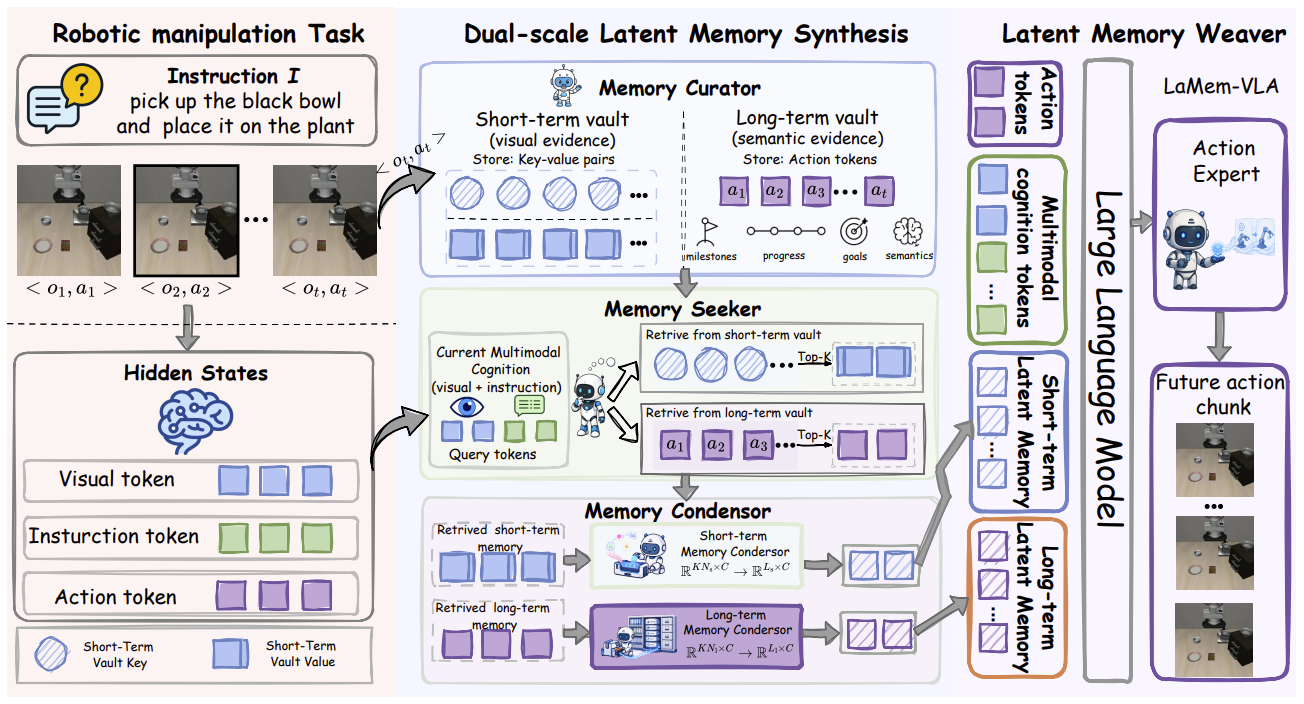
\includegraphics[width=0.99\textwidth]{figs/overview.png}
    \vspace{-10pt}
    \caption{\small{\textbf{The Framework  of \ourmethod.} Given an instruction and the current observation, the vision–language encoder first encodes the inputs into a multimodal representation.   
    The memory curator (\S\ref{sec:curator}) organizes historical experience into dual memory vaults, and the memory seeker (\S\ref{sec:seeker}) then retrieves task-relevant evidence from dual memory vaults based on this multimodal representation.
This retrieved evidence is compressed into fixed-length latent memory tokens by the memory condenser~(\S\ref{sec:seeker}). Finally, the memory weaver~(\S\ref{sec:weaver}) injects these latent memory tokens into the reasoning sequence, producing memory-grounded action tokens that guide the action expert to generate future action chunks.
}}
    \label{fig:overview}
    \vspace{-15pt}
\end{figure}

\subsection{Problem Formulation}
We formulate the robotic manipulation task in VLA models as a language-conditioned  Markovian decision-making problem. 
At each timestep $t$, the VLA policy~\cite{kim2025fine,kim2025openvla,li2024cogact}, $\bm{\Pi}_\theta$ takes  a natural-language instruction $\bm{I}$ and the current visual observation $\bm{o}_t$ as input, and predicts a chunk of future actions for executing the specified task:
\begin{equation}
    \label{eq:problem_formulation}
         \bm{a}_{t:t+H-1} = \bm{\Pi}_\theta(\bm{o}_t, \bm{I}),
\end{equation}
where $H$ denotes the action horizon, and each action $a_t \in {\mathbb{R}}^{7}$ is a 7-DoF end-effector control vector, consisting of 3-DoF relative translation, 3-DoF relative rotation, and a 1-DoF gripper state.

\subsection{\ourmethod Model Architecture}
\noindent\textbf{Motivation.}
The Markovian formulation above in VLA models makes action prediction primarily depend on the instantaneous observation and instruction.
Although effective for short-horizon behaviors, this paradigm can induce a temporal short-horizon bias in long-horizon and temporally dependent manipulation tasks, where historical state transitions, completed subtasks, and task-progress cues are essential for reliable control.
Existing works attempt to augment VLA or visuomotor policies with memory through incorporating explicit episode context into the input~\cite{lin2026hif,jang2025contextvla,li2025cronusvla} or externalized memory bank retrieval~\cite{shi2025memoryvla,sridhar2025memer}.
However, they store the historical memory outside the model’s native token space and consume it as auxiliary policy-side context for action decoding, preventing memory from being fluidly interleaved with the internal reasoning process that jointly perceives, reasons, and forms action intent.
Thus, our \ourmethod reformulates robotic memory as context-native latent memory to bridge this gap.

\noindent\textbf{Overview.}
\ourmethod is an end-to-end native latent memory framework for robotic manipulation that directly weaves dual-scale historical experience into VLA reasoning to refine action generation, as shown in Fig.~\ref{fig:overview}.
At each timestep $t$, given the current visual observation $\bm{o}_t$ and instruction $\bm{I}$, the vision-language backbone embeds them into the visual tokens $\bm{X}_t$ and instruction tokens $\bm{I}$.
Learnable action queries are appended to the token sequence to obtain manipulation-relevant latent action representations.
\ourmethod closes the loop between latent memory reconstruction and action reasoning through four coordinated modules.
First, a \textbf{latent memory curator} dynamically establishes and updates two complementary memory vaults: the short-term memory vault $\mathcal{M}^\text{short}$ stores visual tokens that preserve recent perceptual evidence, while the long-term memory vault $\mathcal{M}^\text{long}$ stores action tokens that preserve semantic and action-continuity evidence across longer horizons.
Second, a \textbf{latent memory seeker} constructs a context-aware query $\bm{Q}_t^\text{con}$ from the current multimodal cognition representation and uses it to retrieve decision-relevant history from the two vaults.
Third, a \textbf{latent memory condenser} distills the retrieved raw memory content and learnable memory tokens into compact latent short-term memory tokens $\bm{M}^\text{short}$ and latent long-term memory tokens $\bm{M}^\text{long}$, respectively.
Finally, a \textbf{latent memory weaver} prepends these two sources of latent memory tokens to the current image and language tokens, forming a memory-augmented VLA input sequence $\bm{S}_t$:
\begin{equation}
    \label{eq:vlm_sequence_overview}
    \bm{S}_t = [\bm{M}^\text{short}; \bm{M}^\text{long}; \bm{X}_t; \bm{I}; \bm{Q}^\text{action}],
\end{equation}
where $\bm{Q}^\text{action}$ denotes learnable action tokens.
The resulting action tokens are then fed into a diffusion-based action expert~\cite{peebles2023scalable} to generate action sequences.


% stitches these generated memory tokens into the VLM reasoning sequence before the action queries are resolved:
% Because $M_p$ and $M_c$ are part of the VLM input sequence, the final action queries can attend to current perception, language instruction, short-term memory, and long-term memory within the same self-attention process.
% The corresponding hidden states are then projected into memory-grounded latent action tokens $Z_{act}$, which condition the downstream action policy to generate temporally aware action chunks.


\subsection{Latent Memory Curator}
\label{sec:curator}
The latent memory curator maintains the historical evidence that will later be retrieved, condensed, and woven into the VLA reasoning sequence.
\ourmethod adopts a 7B-parameter Prismatic vision-language model~\cite{karamcheti2024prismatic} as the backbone, which is further pretrained on the large-scale cross-embodiment real robotic dataset Open-X Embodiment~\cite{o2024open}.
For the current RGB observation, the backbone first extracts visual tokens with its vision encoder~\cite{oquabdinov2,zhai2023sigmoid} and projects them into the language embedding space to obtain final visual tokens $\bm{X}_t\!\in\!\mathbb{R}^{N_\text{i}\times C}$, where $N_\text{i}$ is the sequence length and $C$ is the hidden dimension.
These visual tokens are concatenated with the tokenized instruction and processed by LLaMA-7B~\cite{touvron2023llama}.
We append learnable action queries $\bm{Q}^\text{action}\!\in\!\mathbb{R}^{N_\text{a}\times C}$ to the sequence, and use their output hidden states $\bm{H}^\text{action}$ as compact action representations for downstream action prediction.
The curator factorizes the historical evidence into two memory vaults: a short-term memory vault $\mathcal{M}^\text{short}$ and a long-term memory vault $\mathcal{M}^\text{long}$.

\noindent\textbf{Short-term Memory Vault.}
The short-term memory vault $\mathcal{M}^\text{short}$ stores visual perceptual evidence from the current episode.
The resulting initialized vault is denoted as $\{\bm{m}_\text{s}^i\}_{i=1}^L$, where $L$ specifies its initial capacity.
Each short-term memory unit is represented as a key-value pair $\bm{m}_\text{s}^i=(\bm{k}_\text{s},\bm{v}_\text{s})$:
the key $\bm{k}_\text{s}$ provides a concise retrieval summary of visual evidence, while the value $\bm{v}_\text{s}$ stores the latent short-term memory content.
Specifically, at each timestep, a learnable compression module distills the current visual tokens $\bm{X}_t$ into a compact set of short-term memory tokens, and their mean-pooled representation is used as the retrieval key:
\begin{equation}
    \label{eq:visual_memory_bank}
    \begin{aligned}
        \bm{v}_\text{s} &= \mathcal{C}_\text{s}(\bm{X}_t) \in \mathbb{R}^{N_\text{s} \times C}, &
        \bm{k}_\text{s} &= \mathrm{MeanPool}(\bm{v}_\text{s}) \in \mathbb{R}^{C},
    \end{aligned}
\end{equation}
where $\mathcal{C}_\text{s}$ is an SE-bottleneck compression module~\cite{hu2018squeeze}, and the unit $\bm{m}_\text{s}$ is then appended to $\mathcal{M}^\text{short}$.

\noindent\textbf{Long-term Memory Vault.}
The long-term memory vault $\mathcal{M}^\text{long}$ stores the action hidden states that track task progress and action continuity across long horizons.
At each timestep, the curator directly writes the action hidden states $\bm{H}^\text{action}$  into the vault as one long-term memory unit $\bm{m}_\text{l}$. Unlike the short-term vault, $\mathcal{M}^\text{long}$ is not a key-value bank:
each long-term unit preserves the action hidden state at each timestep, allowing the vault to accumulate task-progress and action-continuity information across the trajectory.

\noindent\textbf{Memory Vault Updating Strategy.}
After a new memory unit is written into its corresponding vault, the memory curator applies a compression strategy only when the number of stored units exceeds the capacity $L$.
For the short-term visual stream, let $\mathcal{M}^\text{short}=\{\bm{m}_\text{s}^i=(\bm{k}_\text{s}^i,\bm{v}_\text{s}^i)\}_{i=1}^{n_\text{s}}$ after insertion.
If $n_\text{s}>L$, we compute the cosine similarity between temporally adjacent keys and select the most redundant adjacent pair:
\begin{equation}
    \label{eq:short_memory_capacity}
    i_\text{s}^* =
    \arg\max_{1 \le i < n_\text{s}}
    \mathrm{cos}(\bm{k}_\text{s}^i,\bm{k}_\text{s}^{i+1}).
\end{equation}
The selected pair is consolidated by averaging both its key and value tokens:
\begin{equation}
    \label{eq:short_memory_merge}
    \begin{aligned}
        \tilde{\bm{k}}_\text{s} &=
        \frac{1}{2}(\bm{k}_\text{s}^{i_\text{s}^*}+\bm{k}_\text{s}^{i_\text{s}^*+1}), \qquad
        \tilde{\bm{v}}_\text{s} =
        \frac{1}{2}(\bm{v}_\text{s}^{i_\text{s}^*}+\bm{v}_\text{s}^{i_\text{s}^*+1}), \qquad
        \tilde{\bm{m}}_\text{s} &= (\tilde{\bm{k}}_\text{s},\tilde{\bm{v}}_\text{s}).
    \end{aligned}
\end{equation}
The two adjacent units are replaced by $\tilde{\bm{m}}_\text{s}$, reducing redundancy while preserving their shared visual evidence. \ourmethod applies the same memory updating strategy to the long-term memory vault. See more details in Appendix.

\subsection{Learning to synthesize latent memory with Dual-scale Vault}
\label{sec:seeker}
\ourmethod does not expose memory vaults to the action policy as raw auxiliary context.
Instead, it treats the two vaults as latent evidence substrates: 
given the current multimodal cognition representation, \ourmethod first retrieves relevant evidence from the two vaults and then reconstructs it into compact memory tokens that are native to the VLA embedding space.
This design decouples memory storage from memory consumption, allowing historical experience to remain flexible in the vaults while entering action reasoning through a bounded latent interface.

\noindent\textbf{Latent Memory Seeker.}
The latent memory seeker retrieves evidence from the memory vaults according to the current multimodal cognition context rather than the visual observation or language instruction alone.
Given the current visual tokens $\bm{X}_t$ and instruction tokens $\bm{I}$, the VLA backbone produces context-aware query $\bm{Q}_t^\text{con}$ that encode the current visual-linguistic cognition. The seeker then appends learnable query slots $\bm{Q}^\text{init}\in\mathbb{R}^{K_\text{q}\times C}$ to $\bm{Q}_t^\text{con}$ and updates only the query slots with a lightweight query builder:
\begin{equation}
    \label{eq:latent_memory_query}
    \bm{Q}_t = \mathcal{B}([\bm{Q}_t^\text{con}; \bm{Q}^\text{init}])[-K_\text{q}:]
    \in \mathbb{R}^{K_\text{q}\times C},
\end{equation}
where $\mathcal{B}$ is a transformer-based query builder (more details in Appendix) and $\bm{Q}_t$ serves as the shared memory hook for both vaults.
We apply masked attention inside $\mathcal{B}$ such that the appended query slots read from $\bm{Q}_t^\text{con}$, while the original multimodal hidden states are not perturbed by the query slots.
The mean-pooled query
$\bm{q}_t\!=\!\mathrm{MeanPool}(\bm{Q}_t)\in\mathbb{R}^{C}$
is used as the global retrieval vector.

The memory seeker then uses $\bm{q}_t$ to retrieve context-relevant units from the short-term vault $\mathcal{M}^\text{short}=\{(\bm{k}_\text{s}^i,\bm{v}_\text{s}^i)\}_{i=1}^{|\mathcal{M}^\text{short}|}$ by cosine similarity:
\begin{equation}
    \label{eq:short_memory_retrieval}
    \begin{aligned}
        \mathcal{I}_\text{s}
        &= \mathrm{Top\!-\!}K
        \left(\{\mathrm{cos}(\bm{q}_t,\bm{k}_\text{s}^i)\}_{i=1}^{|\mathcal{M}^\text{short}|}\right),
        &
        \bm{Z}^\text{short}
        &= \mathrm{Concat}_{i\in\mathcal{I}_\text{s}}(\bm{v}_\text{s}^i)
        \in \mathbb{R}^{KN_\text{s}\times C},
    \end{aligned}
\end{equation}
where $K$ is the number of retrieved short-memory units, and the discrete $\mathrm{Top\!-\!}K$ operation is not optimized by gradient descent.
For long-term memory retrieval, the seeker similarly ranks the units in $\mathcal{M}^\text{long}=\{\bm{m}_\text{l}^i\}_{i=1}^{|\mathcal{M}^\text{long}|}$ via comparing the mean-pooled long-term units with the mean-pooled query $\bm{q}_t$.
It then selects the $\mathrm{Top\!-\!}K$ long-term memory units and stacks them into $\bm{Z}^\text{long}\in \mathbb{R}^{KN_\text{l}\times C}$.
The retrieved sets $\bm{Z}^\text{short}$ and $\bm{Z}^\text{long}$ are passed to the memory condenser below as short-term visual evidence and long-term semantic evidence, respectively, instead of being inserted verbatim into the VLA sequence.


\noindent\textbf{Latent Memory Condenser.}
The retrieved short-term visual evidence $\bm{Z}^\text{short}\in\mathbb{R}^{KN_\text{s}\times C}$ and long-term semantic evidence $\bm{Z}^\text{long}\in\mathbb{R}^{KN_\text{l}\times C}$ often contain redundant historical evidence that is not fully aligned with the current context.
Additionally, directly inserting these lengthy retrieved evidence sequences into the VLA sequence would expand the reasoning context and introduce redundant historical tokens, so the latent memory condenser reconstructs them into fixed-length latent memory tokens and maps them into the VLA reasoning embedding space.
Specifically, we introduce learnable short-term visual memory slots $\bm{T}_\text{s}\in\mathbb{R}^{L_\text{s}\times C}$ and long-term semantic memory slots $\bm{T}_\text{l}\in\mathbb{R}^{L_\text{l} \times C}$, and update them with lightweight memory formers conditioned on the context query tokens $\bm{Q}_t\in\mathbb{R}^{K_\text{q}\times C}$ and the retrieved evidence:
\begin{equation}
    \label{eq:memory_condensation}
    \begin{aligned}
        \bm{M}^\text{short} &= \mathcal{F}_\text{v}([\bm{Q}_t; \bm{Z}^\text{short}; \bm{T}_\text{s}])[-L_\text{s}:], &
        \bm{M}^\text{long} &= \mathcal{F}_\text{c}([\bm{Q}_t; \bm{Z}^\text{long}; \bm{T}_\text{l}])[-L_\text{l}:],
    \end{aligned}
\end{equation}
where $\mathcal{F}_\text{v}$ and $\mathcal{F}_\text{c}$ denote lightweight transformer-style memory formers similar to $\mathcal{B}$ for the short-term visual and long-term semantic memory, respectively.
The resulting $\bm{M}^\text{short}$ and $\bm{M}^\text{long}$ are query-conditioned latent short-term and long-term memory tokens in the same $C$-dimensional embedding space used by VLA reasoning.
This fixed-length property makes the injected memory independent of the retrieval size while preserving evidence from the two vaults.

\subsection{Interweaving Memory into Action Reasoning in Latent Space}
\label{sec:weaver}
\noindent\textbf{Latent Memory Weaver for Guidance Generation.}
Rather than passing the condensed memory tokens to a policy head as external conditioning alone, the latent memory weaver injects the synthesized memory into the VLA reasoning sequence before action queries are resolved.
Although the two types of latent memory differ in provenance, they share the same latent token interface.
Given the condensed short-term memory tokens $\bm{M}^\text{short}$, long-term memory tokens $\bm{M}^\text{long}$, the weaver constructs the memory-augmented VLA input sequence $\bm{S}_t$:
\begin{equation}
    \label{eq:memory_weaver}
    \begin{aligned}
        \bm{S}_t &=
        [\bm{M}^\text{short} + \mathbf{1}_{L_\text{s}}\bm{b}_\text{s}^\top;
        \bm{M}^\text{long} + \mathbf{1}_{L_\text{l}}\bm{b}_\text{l}^\top;
        \bm{X}_t; \bm{I};
        \bm{Q}^\text{action}],  &      \bm{Z}^\text{action}= \mathrm{VLM}(\bm{S}_t)[-N_\text{a}:],
    \end{aligned}
\end{equation}
where $\bm{b}_\text{s},\bm{b}_\text{l}\in\mathbb{R}^{C}$ are learnable source embeddings for the two memory streams, and $\mathbf{1}_{L_\text{s}},\mathbf{1}_{L_\text{l}}$ are all-one column vectors that broadcast them over the short-term and long-term memory tokens.
Because the two sources of memory tokens are part of the model input sequence, they participate in self-attention with the current observation, language instruction, and action queries.
Thus, the resulting $\bm{Z}^\text{action}$ inside the model reasoning process is formed as memory-grounded action tokens rather than by external policy-side fusion.

\noindent\textbf{Diffusion-based Action Expert.}
After the vision-language backbone produces the memory-grounded action tokens $\bm{Z}^\text{action}$, the diffusion-based action expert decodes them into a continuous action chunk.
Following the diffusion policy~\cite{chi2025diffusion}, we formulate action generation as conditional denoising over an action chunk.
Let $\bm{a}_{t:t+H-1}^{0}$ denote the clean expert action chunk and $\bm{a}_{t:t+H-1}^{n}$ denote its noisy version at diffusion step $n$.
At each denoising step, the noisy action tokens are injected with the diffusion timestep embedding and conditioned on action tokens $\bm{Z}^\text{action}$.
% , while attending to $\bm{M}^\text{short}$ for fine-grained short-term visual evidence and $\bm{M}^\text{long}$ for long-term task-progress and action-continuity cues.

The diffusion expert $\epsilon_\theta$ is trained with mean squared error (MSE) loss to predict the injected noise under these action and memory conditions:
\begin{equation}
    \label{eq:diffusion_loss}
    \mathcal{L}_\text{action}
    =
    \mathbb{E}_{n,\epsilon}
    \left[
    \left\|
    \epsilon -
        \epsilon_\theta(\bm{a}_{t:t+H-1}^{n}, n, \bm{Z}^\text{action})
    \right\|_2^2
    \right].
\end{equation}
During inference, DDIM sampling~\cite{songdenoising} iteratively denoises the action chunk under the same conditions, producing history-aware continuous $7$-DoF control actions.
